\chapter{Lateral histograms}
This chapter treats of lateral histograms, which in our case simplify to row and column sums of the image. Although being very simple in principle, the lateral histograms show as a strong and robust method for EPOH and ECH detection. The largest part of its success, however, depends on the methods for estimating the period from the histograms. We present several such methods and their comparison.

\section{Lateral histograms applied to ionograms}
Lateral histograms are a little more general notion than we need in ionograms. We first provide the general definition and then we look for the more specialized one. We also observe a great simplification brought to this method by the nature of ionograms.

\subsection{Definition}
The general definition of lateral histograms is that ``the lateral histogram technique involves projecting an image on two or more axes by summing pixel intensities [\ldots] and using the resulting histograms to identify objects in the image.'' \citep{Davies2004} As can be seen, the title ``histograms'' does not have exactly the common meaning (counts of points with similar values). The slightly changed definition uses sums instead of counts and the ``similar values'' mean the same position with respect to the chosen axis.

To detect EPOHs and ECHs it is sufficient to take into account only the vertical and horizontal axes (whereas the definition allows for arbitrary axes). This is because EPOHs are strictly vertical lines and ECHs strictly horizontal. Summing up rows or columns, it can be clearly seen that in most cases the harmonic echoes generate high peaks in these histograms. The height of the peak corresponds to the length of the harmonic echo line as can be seen in Fig. \ref{fig:colSums}. 

\begin{figure}
	\centering
	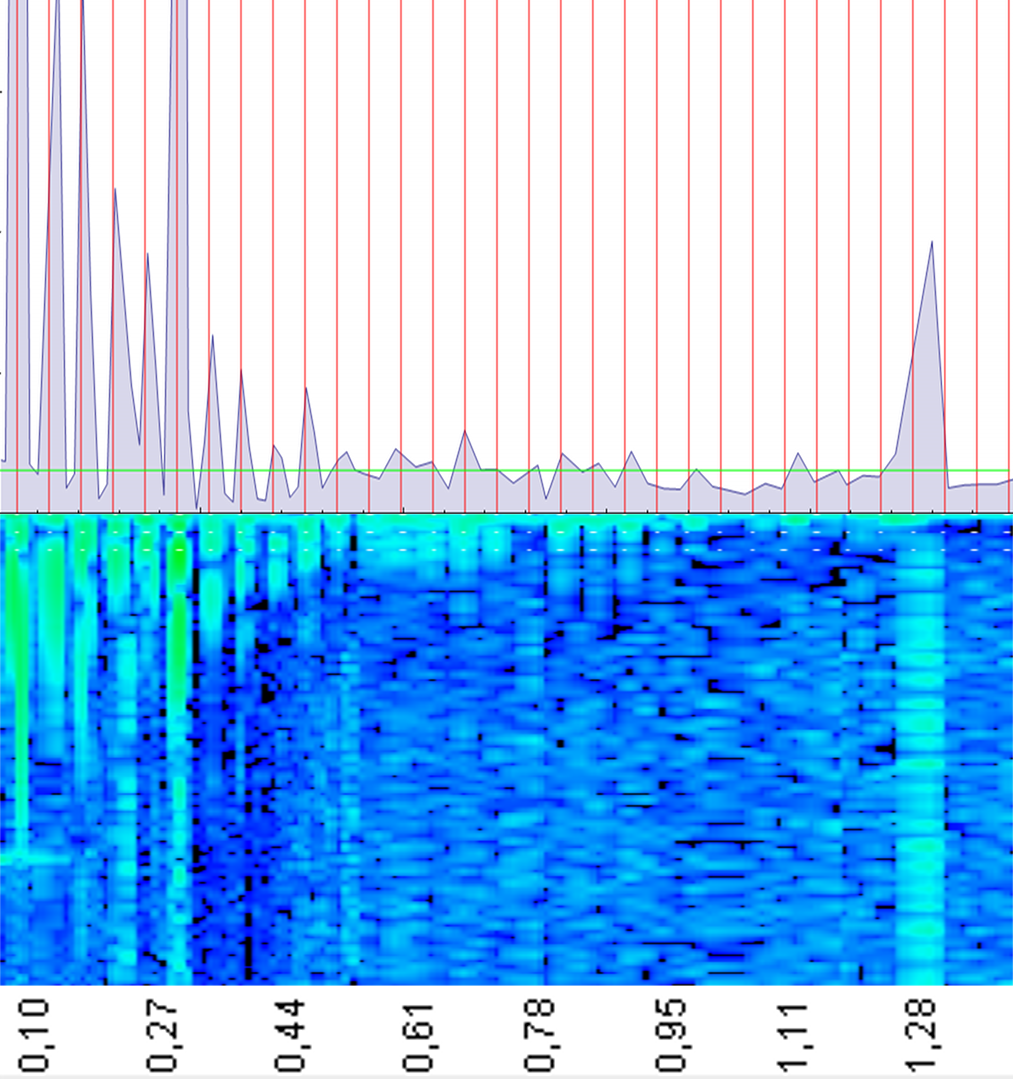
\includegraphics[width=140mm]{images/column_sums_orbit_3974_000.png}
	\caption{The column sums of a part of ionogram. The ionogram below is displayed along the sounding frequency scale in MHz. The top part shows the column sums at the frequencies from ionogram. The red lines represent the harmonics of the manually measured repetition period. They very closely correspond to the peaks in column sums. The green horizontal line denotes the mean value of the sums.}
	\label{fig:colSums}
\end{figure}

\subsection{Simplification in the case of ionograms}
The general definition assumes we are looking for point-like structures (given by 2~coordinates) and thus requires computing the histogram along at least two axes. From two histograms both 2D coordinates can be determined, but often there are ambiguities in the solution (for features overlapping in the direction perpendicular to an axis) \citep[chap.~13]{Davies2004}. The removal of such ambiguities is not trivial. 

Fortunately, in the ionogram case, only one axis is sufficient for every feature, since we are not interested in the length of the echo lines. Having the one histogram, detection of its peaks is all that is needed. Not all peaks in the histogram correspond to a harmonics line, some lower of them can be caused by noise.

\section{Implementation}
We implemented a feature detector using the lateral histograms technique on evenly sampled ionograms. It can be found on the attached CD in directory \texttt{programs/detector-summing}. See \nameref{sec:running} for information on how to run it. 

\subsection{Finding and filtering the peaks}
Due to the properties of both EPOH and ECH we can reduce the problem to working on the left half of ionograms. It may happen that some EPOHs stretch beyond the half, but in such cases there have to be lots of other harmonic lines in the left part (since the harmonics are the stronger the closer they are to the base frequency). As all ECHs start at the left border and usually are not very long, cutting the image in half is also possible.

As stated above, not all peaks in the histogram belong to the harmonic echoes. In order to find only the high peaks, we first filter out \n[\%]{50} of the row/column sums with the lowest values. We should be able to detect periods of length 2 bins, which would give just the \n[\%]{50} threshold. As can be derived from \citep[p.~3]{Akalin2010}, detecting periods less than \n{2.5} bins is impractical in the time domain, which yields threshold of \n[\%]{60}. As echoes in the frequency domain have to be sparser (due to the quasi-logarithmic spacing and quantization to bins), we can use this threshold, too.

With the uninteresting values filtered out (by setting them to zero) we can proceed to finding the peaks. The algorithm is rather simple, it just treats as a peak every data point with both neighboring values lower or equal to it. Once it finds a peak it zeroes out both non-increasing sequences neighboring to it (to get rid of non-strict maxima). What remains are the highest local maxima of the histogram.

\subsection{Determining the period}
In an ideal case the set would contain all the harmonic lines positions and no more. In practice, noise and data inaccuracies introduce some false peaks. As a heuristic to tell if a peak comes from harmonic lines, we can look at its height. The echo lines are often long and have their values more than 10~times higher than the background around them. Both these facts contribute to greater values of the row/column sums. For EPOH, if there are some ECH lines or an IE in the image, they disappear in the peaks list. It is because they are perpendicular to the EPOH lines and so may fill up the space between EPOHs, but in the frequency domain, their contribution is relatively small in comparison with the contribution of the EPOH lines. Ground echoes are almost completely discarded by cutting the ionogram in half. Similarly, while detecting ECH lines, the EPOH lines should cause no trouble. However, an IE can cause problems because it usually adds a very high and broad peak to row sums. This is a caveat of using this method to detect ECHs.

We should also be able to recognize when there are no data of interest in the ionogram. Using just row/column sums it would have been, however, more a statistical than algorithmic decision. We could say what levels of row/column sums mean no feature is present, or we could try to measure the ``ruggedness'' of the histogram to tell if there are some peaks, but we chose to rather not do such estimates and instead allow false positive detections. Removal of the false positives can be done later by comparing to the results of other methods more suitable to tell that a feature is not present at all. 

So we have the peaks and their heights as heuristics (telling us the probability of them to come from a line of interest). Combining these, we are finally able to estimate the repeat frequency. The last remaining task is to find a method taking peak positions and their weights and computing the most probable period. The following section lists three implemented methods.

\section{Period estimation}
A period estimation method has to count with the fact that there are some peaks missing and some of them are extra. It should hold that the extra peaks have relatively low weights. On the other hand, the ``regular'' peaks can also have low weights.

\subsection{Periodograms}













